49. \begin{figure}[ht!]
\center{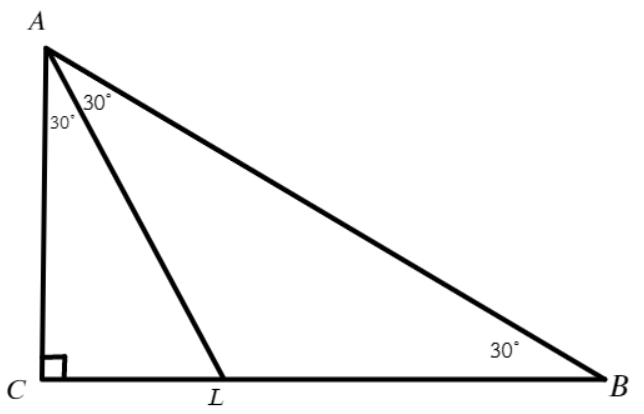
\includegraphics[scale=0.35]{g49.png}}
\end{figure}\\
Если внешний угол при вершине $B$ равен $150^\circ,$ то $\angle B=180^\circ-150^\circ=30^\circ.$ Тогда $\angle A=90^\circ-30^\circ=60^\circ$ и $\angle CAL=\angle LAB=30^\circ$ (так как $AL$ --- биссектриса). В прямоугольном треугольнике $CAL$ катет $CL$ лежит напротив угла в $30^\circ,$ поэтому $CL=\frac{1}{2}AL=\frac{1}{2}\cdot3=1,5$см. В треугольнике $LBA$ углы при стороне $BA$ равны, значит он равнобедренный и $BL=AL=3$см. Таким образом, $BC=CL+BL=1,5+3=4,5$см.\\
